

\maketitle
\documentclass[12pt,a4paper]{article}

\usepackage[a4paper,margin=1in]{geometry}
\usepackage{graphicx}
\usepackage{float}
\usepackage{hyperref}
\usepackage{enumitem}
\usepackage{xcolor}
\usepackage{listings}
\usepackage{titlesec}

\hypersetup{
    colorlinks=true,
    linkcolor=blue,
    urlcolor=blue
}

\begin{document}

%====================================================
% TITLE PAGE
%====================================================

\begin{titlepage}

\centering


\includegraphics[height=4cm]{logo.jpeg}

\vspace{1cm}

{\Large GISMA University of Applied Sciences}

\vspace{0.8cm}

{\Huge \textbf{Computer Science Portfolio Project}}

\vspace{0.5cm}

{\Large B201D Computer Science Lab}

\vspace{2cm}

\textbf{Student Name:}\\
Jahanvi

\vspace{0.5cm}

\textbf{Student ID:}\\
GH1040369

\vspace{0.5cm}

\textbf{Professor Name:}\\
William Baker Morrison

\vfill

\today

\end{titlepage}

%====================================================
% TABLE OF CONTENTS
%====================================================

\tableofcontents
\newpage

%====================================================
\section{Introduction}

The report presents the design, development, and evaluation of my personal portfolio website.
The purpose of this project is to create a online portfolio that showcases my technical skills, academic achievements, and projects, applying for internship or working student positions. My personal portfolio website mainly consists of three components a GitHub repository which contains the project files, a website using GitHub Pages, and a professional curriculum vitae (CV) created in LaTeX.
The website was developed using HTML, CSS and JavaScript because they provide a strong understanding for building a website. This report tells about objects of the project, structure of website and GitHub, which technologies i have used, the implementation process, and future outcome.
%====================================================
\section{Project Objectives}

The project was developed using various objectives 

\begin{itemize}
    \item Develop a professional portfolio website.
    \item Created a CV using LaTeX.
    \item Demonstrate knowledge of HTML, CSS, and JavaScript.
    \item Git and GitHub were used for version control.
    \item  Hosted a website using GitHub Pages.
    \item Present technical skills and projects effectively.
\end{itemize}

%====================================================
\section{Portfolio Overview}

\subsection{Portfolio Website}

\url{https://jaanii-code.github.io/Computer-science-lab-project/}

\subsection{GitHub Repository}

\url{https://github.com/jaanii-code/Computer-science-lab-project}


The portfolio website presents my educational background, technical skills, selected projects, and contact details. It was designed concisely because visitors or hiring managers can understand the type of work i have completed and the knowledge i  have gained from my field. In addition, by building the website , I learned not only the theoretical understanding but also to translate the ideas into the online website.

The website was designed to be responsive, easy to navigate, and visually appealing for creating a professional first impression.

%====================================================
\section{Website Structure}

The website consists of several sections, each section was designed in a structured way to present a specific type of information, which shows clearly and professionally portfolio.

\subsection{Home Section}

The homepage introduces visitors to the portfolio, the primary purpose is to provides a summary of who I am. The homepage was designed to be concise so that visitors can understand the site without any complexity. Moreover, my resume is available on the portfolio website which is created in LaTeX.

\begin{figure}[H]
\centering
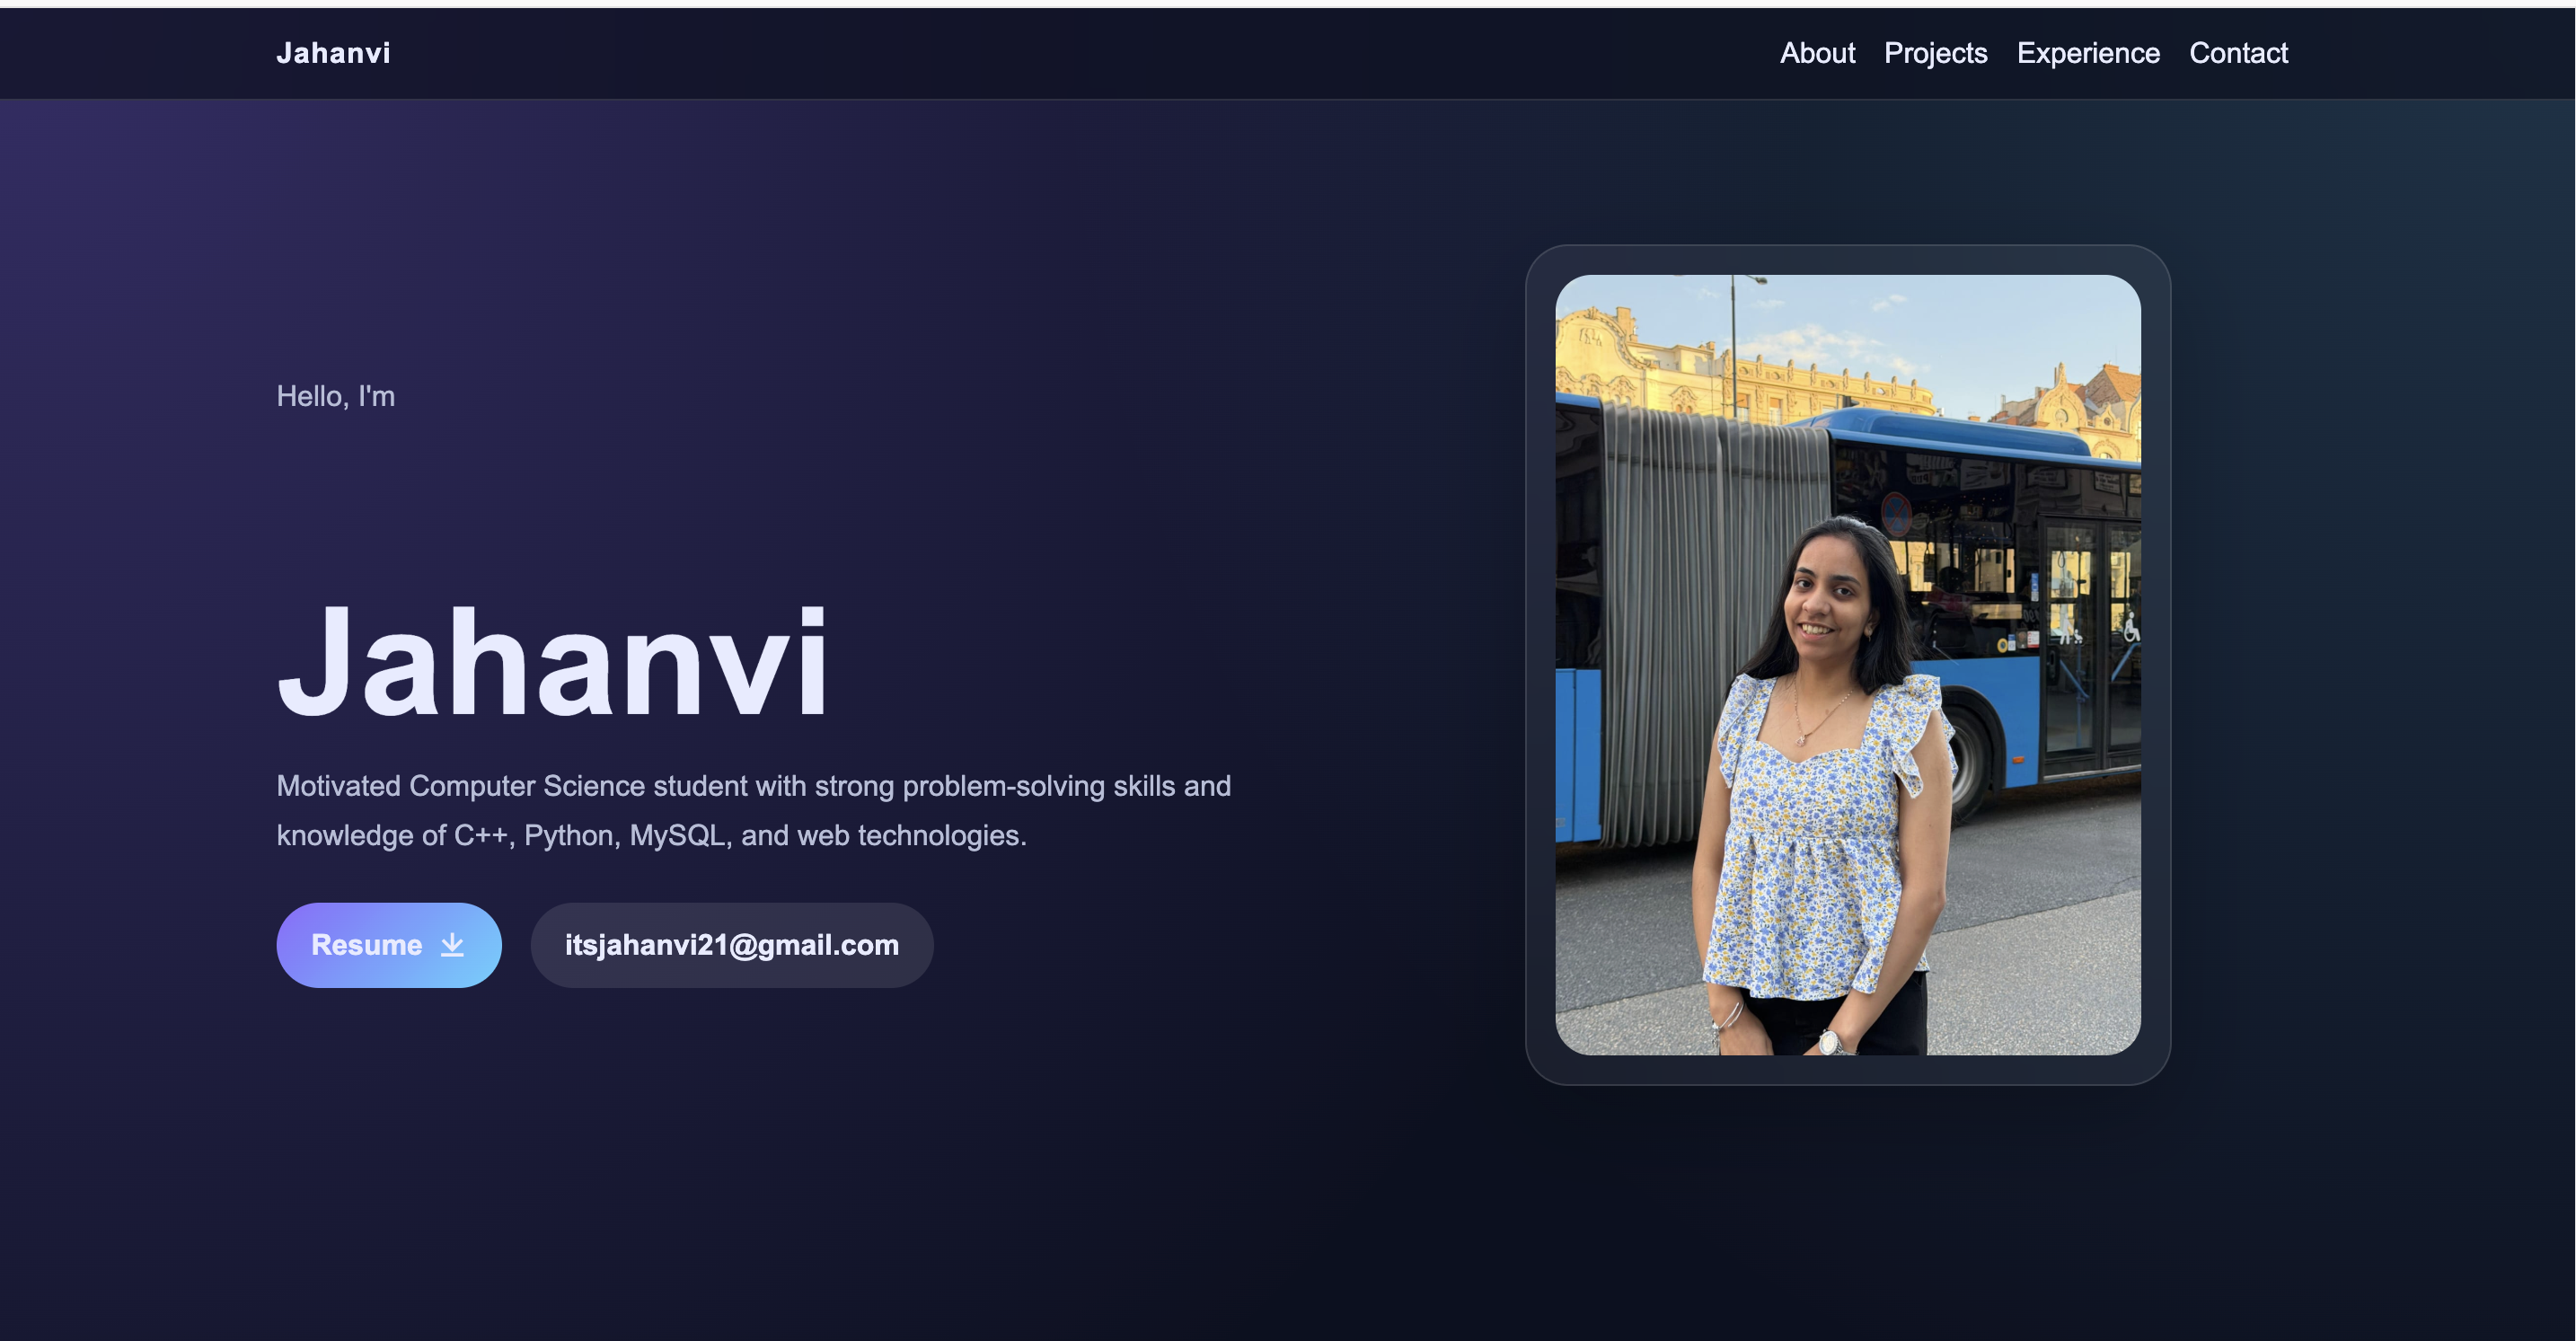
\includegraphics[width=0.9\textwidth]{home.png}
\caption{Homepage of the Portfolio Website}
\end{figure}

\subsection{About Me}

This section contains information about my educational background, interests, and career goals. . It is consider to be important as it helps employers to see the technical skills as they are also interested in motivation, and to present oneself professionally.


\subsection{Skills}

The skills section highlights my technical capabilities including programming languages, development tools, and relevant  technologies. It allows to quickly identify the abilities I have gained in the area I have worked practically, while it helps the people who are visiting my site to match the technical requirements according to their preferences, which makes it  easier without going into deeper sections.

\begin{figure}[H]
\centering
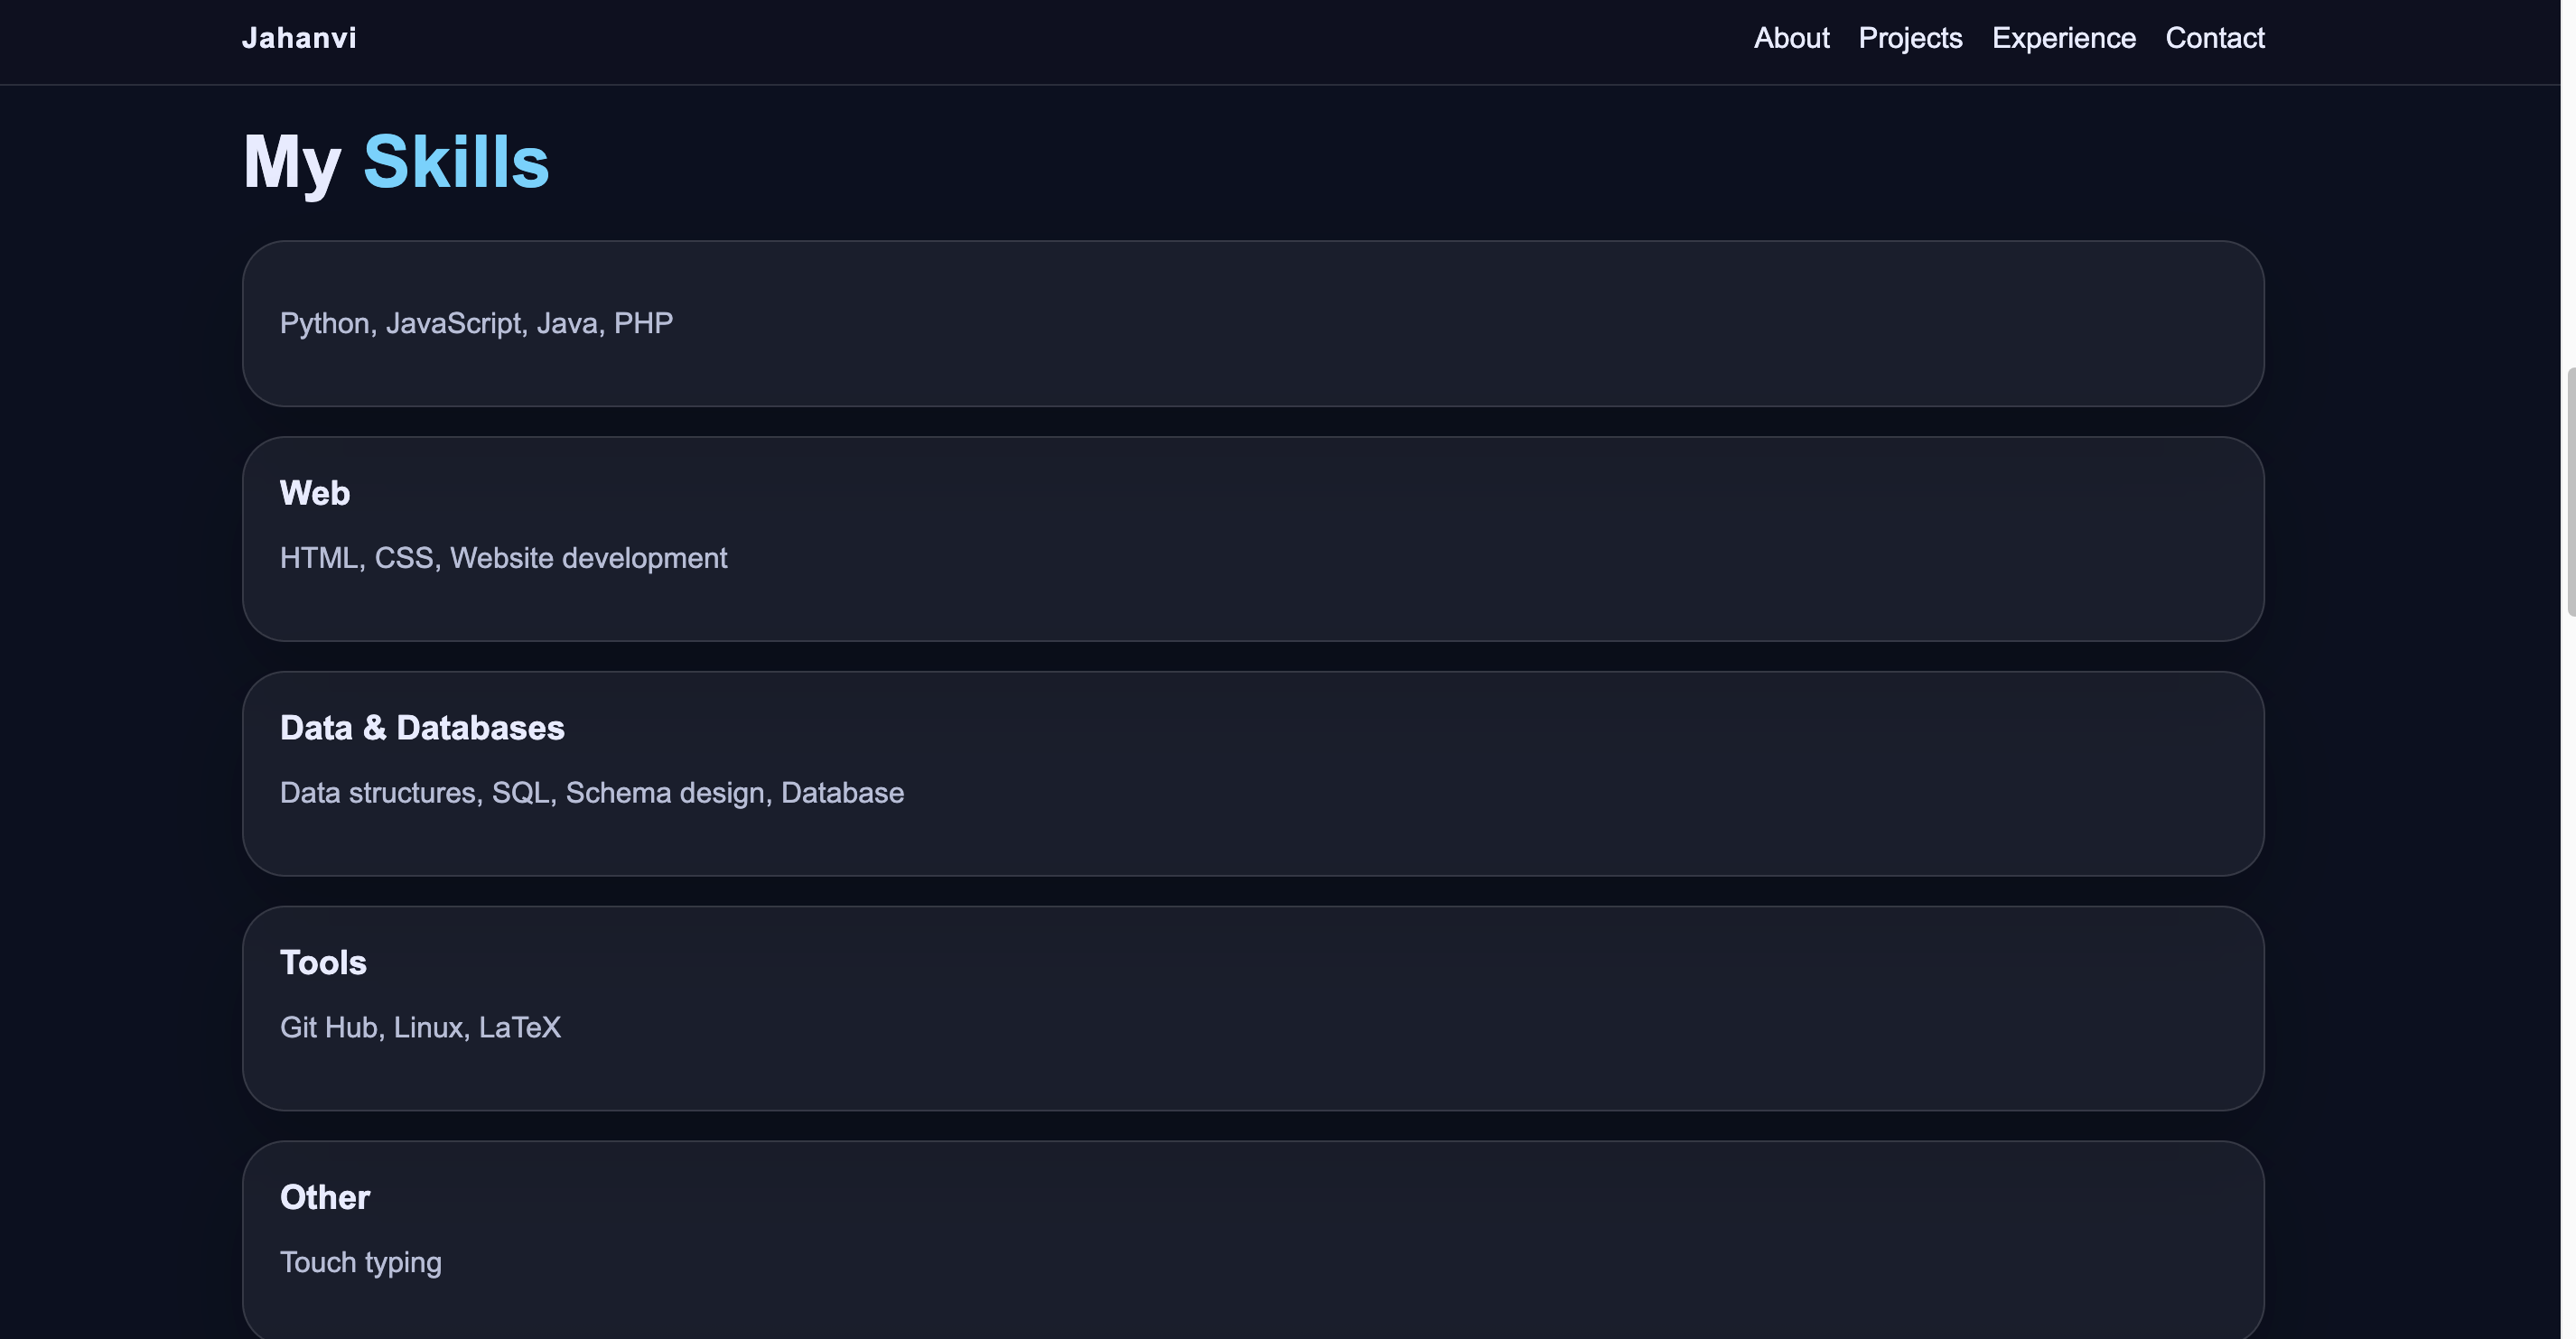
\includegraphics[width=0.9\textwidth]{skill.png}
\caption{Skills Section}
\end{figure}

\subsection{Projects}

The projects section is one of the most important part of the portfolio as it includes about experiences or examples of work . Rather than stating the technical skills , it also includes that how all the skills i have applied in practice. I have worked in selected projects to demonstrate the problem-solving skills, and technical skills i have learned. 
\begin{figure}[H]
\centering
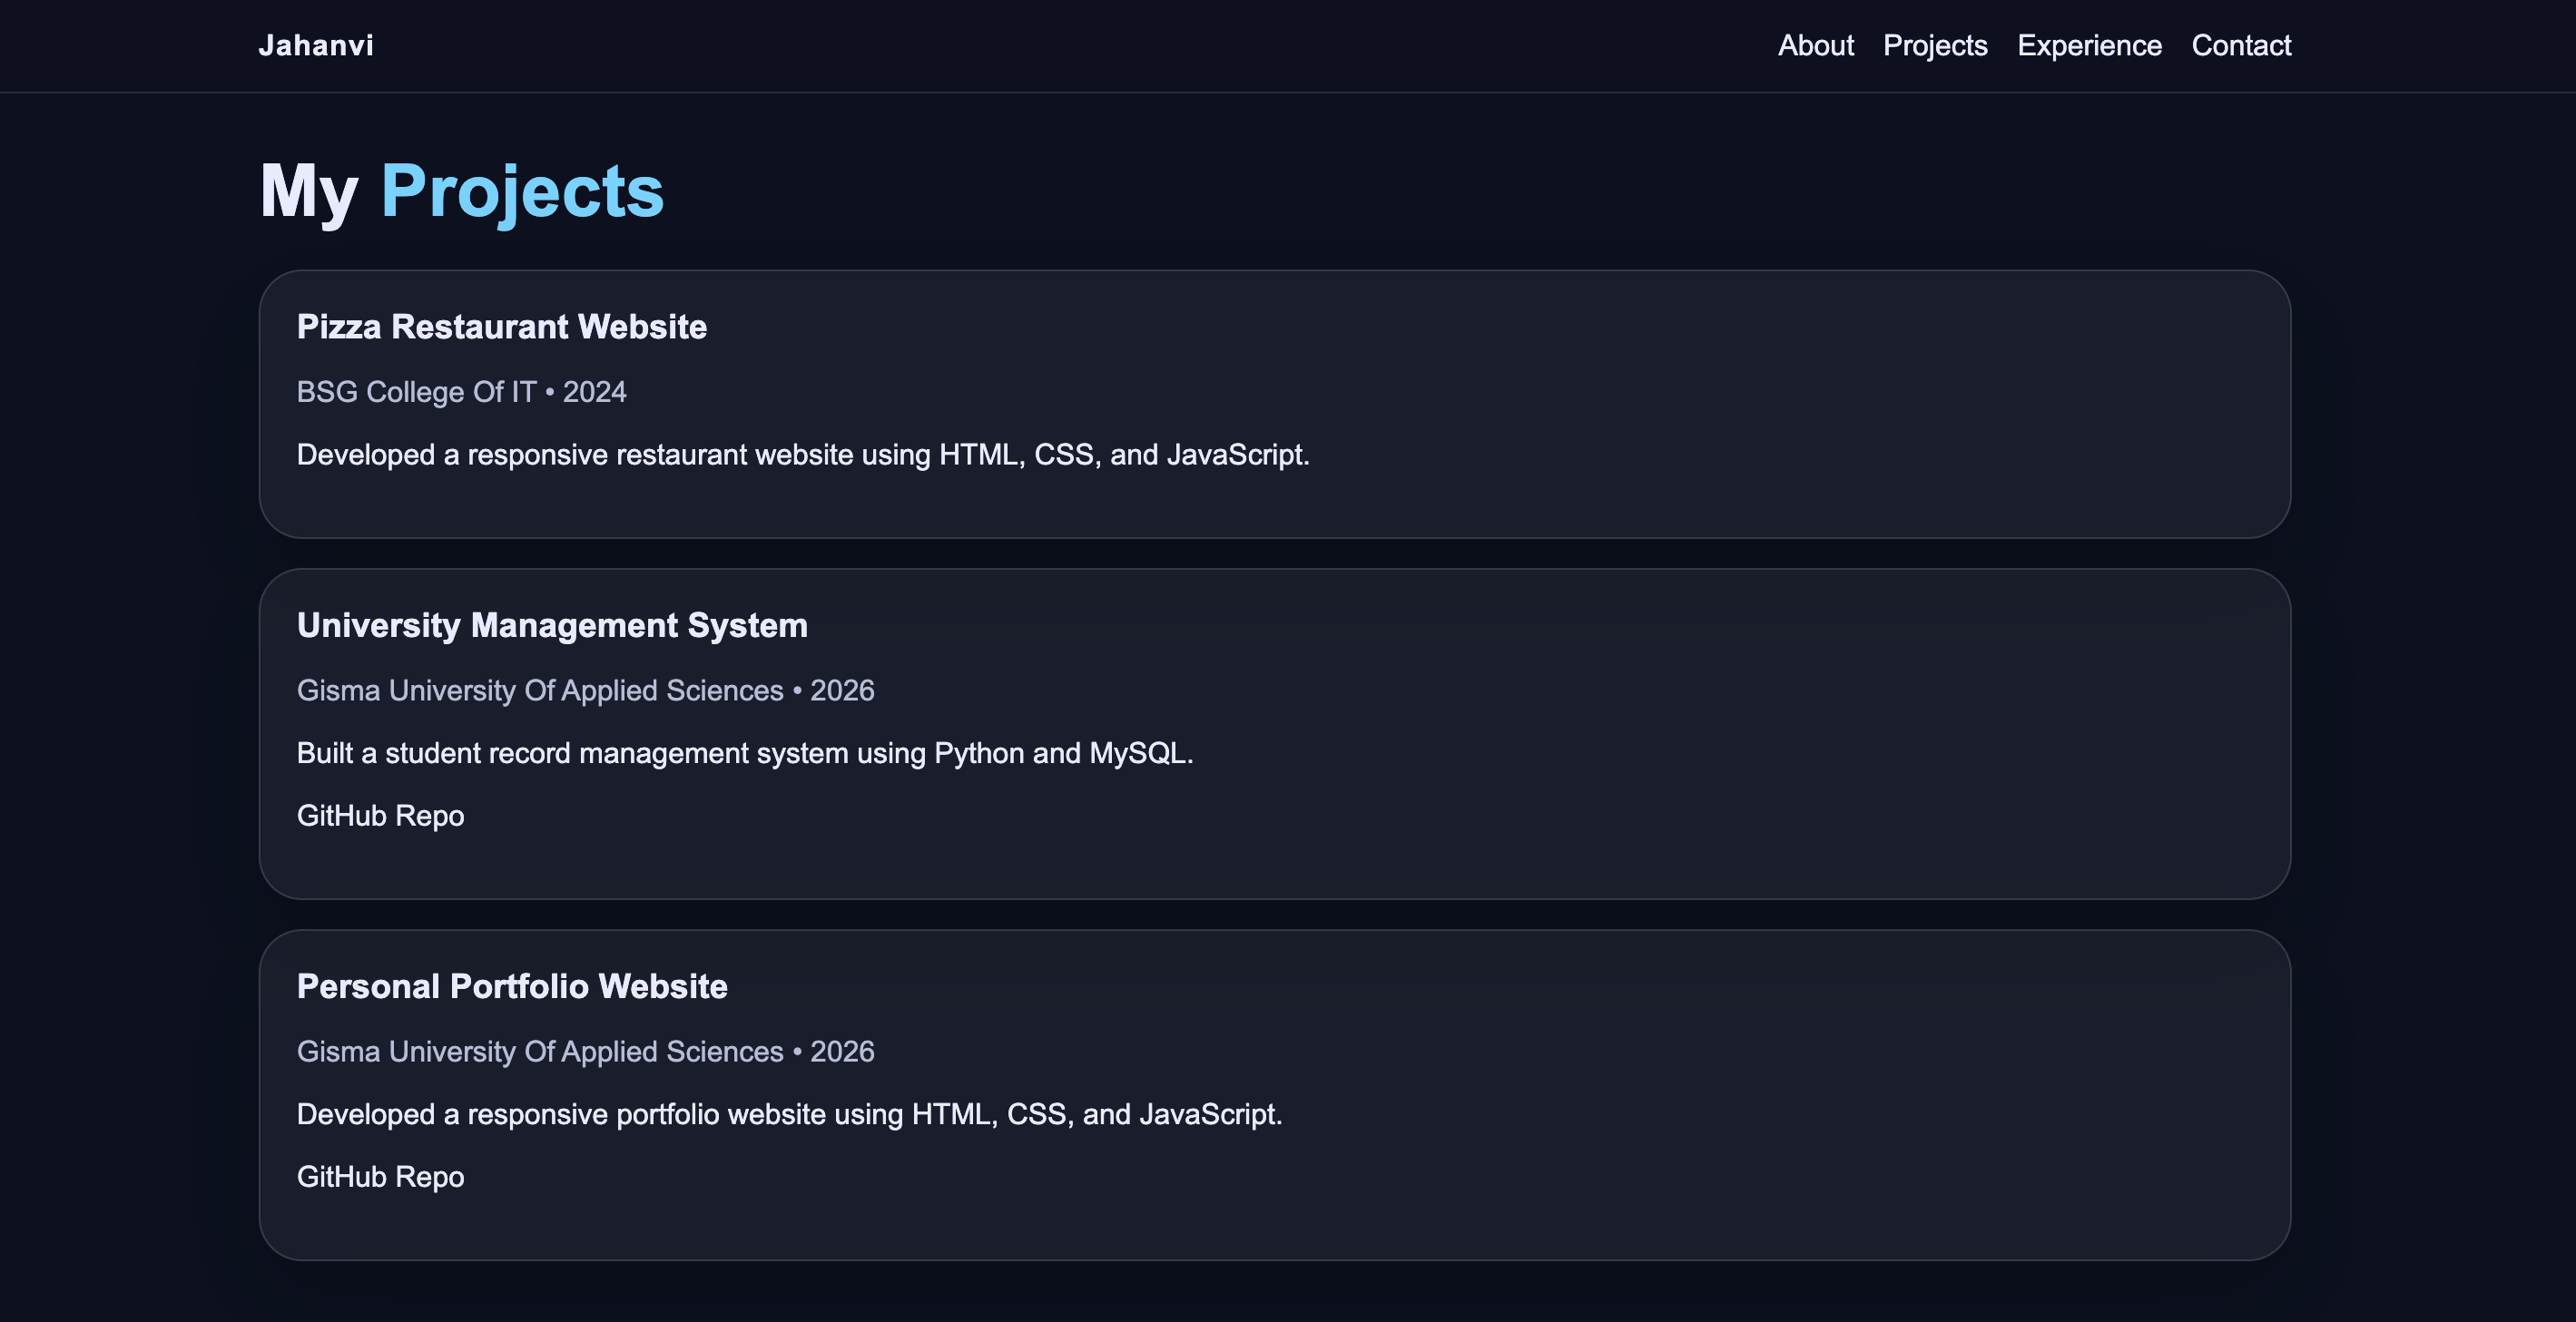
\includegraphics[width=0.9\textwidth]{projects.png}
\caption{Projects Section}
\end{figure}

\subsection{Contact Section}

The contact section provides information that allows employers, collaborators, or other visitors to reach me. Including this information is mandatory as the website not only contain the information but also the communication opportunities. 

%====================================================
\section{GitHub Repository Structure}

The GitHub repository is organized, and separating the files according to the project so that it is easier to understand or update in the future.

\begin{verbatim}
Computer-science-lab-project/
|
|-- index.html
|
|-- assets/
|   |-- images/
|   |-- logo.jpeg
|   |-- css/
|   |-- js/
|   | cv/
|   |-- cv.tex
|   |-- cv.pdf
|-- website.txt
|-- README.md
\end{verbatim}
The \textbf{index.html} contains the main text of the portfolio website . The \textbf{style.css }file was used to control the appearance of website, including layout, fonts and overall design, while \textbf{script.js} provides interactive behavior, improve the webpage where needed. The \textbf{assets} directory stores supporting files such as images and logo. The cv folder contains both the LaTeX source file and the generated PDF version of the CV, which makes this to maintain and update the document efficiently. Lastly, the \textbf{README.md} file tells the  documentation for the repository and helps visitors to know about the project .This structure reflects a separation of concerns, where content, styling, behavior, and documentation are kept distinct. 


%====================================================
\section{Technologies Used}
A range of technologies were used in building-up the portfolio website. Each technology has its own role:
\subsection{HTML}

HTML was used for the structure of the website. It provided all the sections headings, paragraphing, links and images. 

\subsection{CSS}

CSS was used to control the visual design of the website including colors, spacing, fonts, and layout. It also implement the responsive design so that the website can fit into different screen sizes.

\subsection{JavaScript}

JavaScript was used to add interactive functionality and improve the user experience. Even in my simple portfolio website it helps to enhance usability by making the components more dynaminc.

\subsection{Git}

Git was used for version control throughout development.

\subsection{GitHub}

GitHub was used for hosting source code and managing project versions, from this the project was updated in an easy manner .

\subsection{GitHub Pages}

GitHub Pages was selected because it provides a simple,free and effective way for hosting static websites directly from GitHub repository.

\subsection{LaTeX}

LaTeX was used to create a professional curriculum vitae and to prepare the technical documentation. It was used because it enables precise formatting, and structured documentation output for professional contexts.
%====================================================
\section{Design Decisions}

Several design decisions were made to ensure that portfolio should be professional , usable and appropriate for the visitors who sees my portfolio website.

\subsection{Responsive Design}

Responsive design techniques were implemented as it is considered to be important because someone ´can access the portfolio from other devices such as laptops, tablets and smartphones. This reason meant that layout design be adjusted to different sizes that text as well as the designs remains same.

\subsection{Navigation Layout}

A simple navigation menu was chosen to allow users to access content quickly between the sections of the site. A simple and straightforward navigation menu helps to reduces the load and improves the overall experience. 

\subsection{Color Scheme}

A professional and minimalist color palette was selected to improve readability and clean visual appearance. The chosen color also helps to be more formal or professional tone, which make this appropriate for a portfolio intended for hiring managers. 

\subsection{Typography }

Clear and readable typography was used to ensure that users can easily engage with the content. Spacing, font sizes, and contrast allows to read easily. Also, good typography helps to maintain the professional quality of portfolio website.

\subsection{GitHub Pages Deployment}

GitHub Pages was chosen because it integrates directly with GitHub repositories and simplifies the publishing process. This decision was made to smooth the workflow from development to deployment. 
Overall, these all designs were made to create the website more functional, visually coherent and meet with expectations of technical portfolio.

%====================================================
\section{Implementation Process}

The project followed the development structured process which consist of several stages, starting with the planning, and concluding with testing to ensure that the project remain manageable and also the final outcome met the required objectives. 
First, the structure was designed by creating most important sections in professional website, such as homepage, about me , skills, project and contact information. After this, the visual layout was designed to focus on simplicity, clarity, and user-friendly navigation. The HTML structure was developed to website's content, layout and overall page documentation. Moreover, completing the structural thing was complete, CSS was used to style the data page, visual design of the site. JavaScript was then implemented to add interactive things which enhances the users experiences. Apart from this, CV was created in LaTeX to ensure a well-structured document. After all the implementations, all files are uploaded in GitHub, and the website was deployed through GitHub Pages. At last, improving the site, fixing issues, or testing was involved where necessary.  


%====================================================
\section{Evaluation and Reflection}

\subsection{Strengths}

The portfolio demonstrates several strengths. One of its main strength is professional appearance, which makes it easier for the hiring managers, or users to navigate each section in an accessible and organized way to get the information. Another strength is responsive design, which supports ability across different devices.
\subsection{Weaknesses}

Despite these strengths, the portfolio website has limitations. One limitation is small number of showcased projects, which reduces the technical evidence to the users. Another limitation, the features such as fully working contact form are not implemented. In addition, the level of interactivity remains basic. 

\subsection{Challenges Faced}

The development process presented several challenges, first, I struggled with using LaTeX to style a professionally formatted CV. Rich in features though hard to use, and I had some syntax problems that did not allow me to style. Trial and error – eventually, I was able to obtain a clean, styled resume. Additionally, the challenge was deploy a website correctly using GitHub, especially in relation to repository structure and public hosting settings.


\subsection{Learning Outcomes}

Developing this portfolio gave me hands-on experience with front-end web development using HTML, CSS, and JavaScript, as well as technical documentation and deployment using GitHub Pages. It also taught me how to document and present projects professionally, including code and documentation. These experiences are highly transferable to my future career as a data analyst, front- end developer, or scholarly publisher. Above all, this project taught me how to have confidence presenting myself online—technologically and visually.


%====================================================
\section{Conclusion}
This project successfully achieved its core objectives by developing a professional computer science portfolio website together with a supporting GitHub repository and LaTeX CV. It also provides a professional structure, which can be applied in internships, working student positions, and future employment opportunities.
The portfolio demonstrates skills in web development, version control, deployment, and technical documentation. The project provided valuable experience in planning, structuring, implementing, and evaluating a technical solution. As a result, it strengthened both my practical development skills and my understanding of how to present technical work in a professional format. In the future, I plan to further develop this project with dynamic features, more interactive graphs, and even incorporate it into my class work or internship projects.

%====================================================


\end{document}
